\documentclass{article}
\usepackage{standalone}
\usepackage{tikz}
\begin{document}
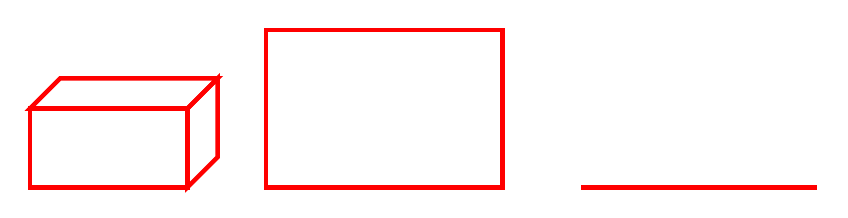
\begin{tikzpicture}
    \begin{scope}
	\pgfmathsetmacro{\cubex}{2}
	\pgfmathsetmacro{\cubey}{1}
	\pgfmathsetmacro{\cubez}{1}
	\draw[red,ultra thick] (0,0,0) -- ++(-\cubex,0,0) -- ++(0,-\cubey,0) -- ++(\cubex,0,0) -- cycle;
	\draw[red, ultra thick] (0,0,0) -- ++(0,0,-\cubez) -- ++(0,-\cubey,0) -- ++(0,0,\cubez) -- cycle;
	\draw[red, ultra thick] (0,0,0) -- ++(-\cubex,0,0) -- ++(0,0,-\cubez) -- ++(\cubex,0,0) -- cycle;
    \end{scope}
    \begin{scope}[xshift=1cm,yshift=-1cm]
	\draw[red,ultra thick] (0,0) rectangle (3,2);
    \end{scope}
    \begin{scope}[xshift=5cm,yshift=-1cm]
	\draw[red,ultra thick] (0,0) -- (3,0);
    \end{scope}
\end{tikzpicture}
\end{document}
